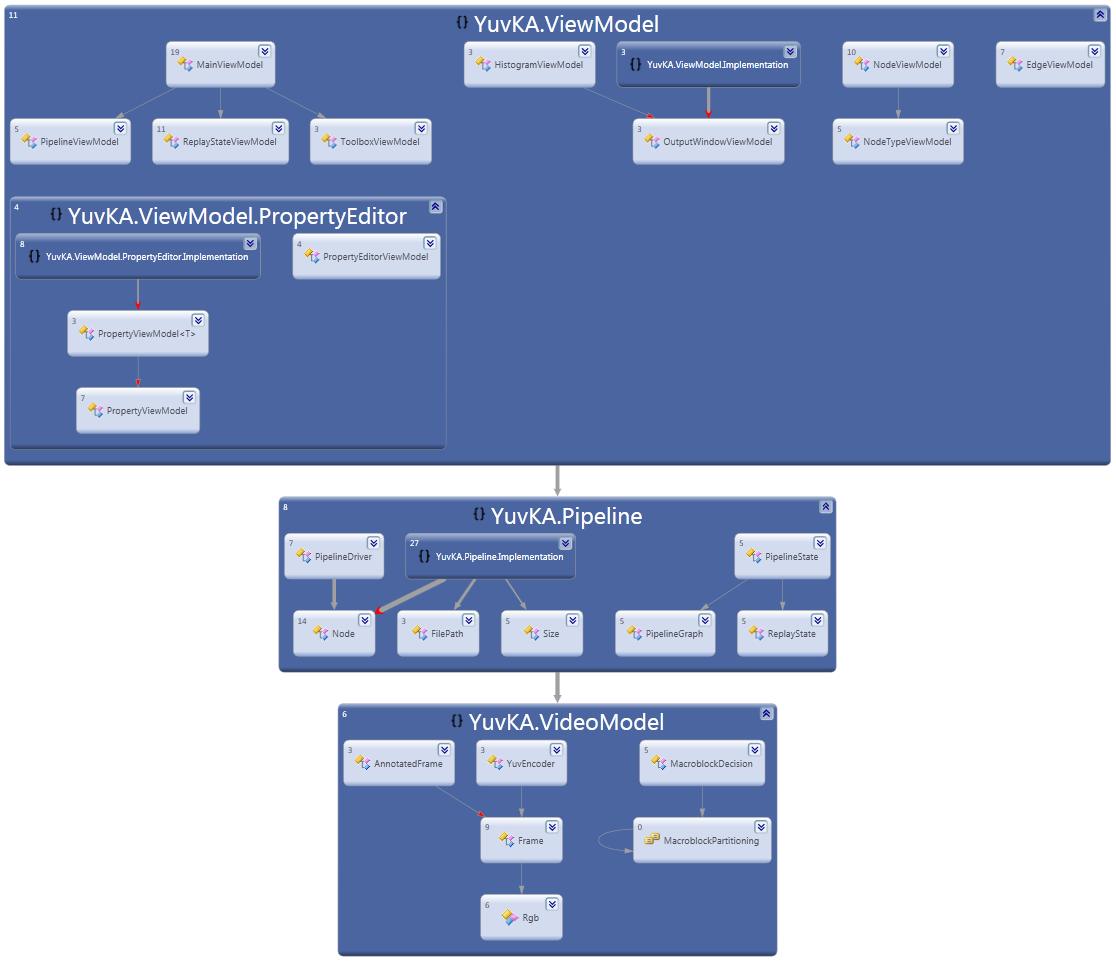
\includegraphics[width=\textwidth]{Diagrams/namespacedependencies.png}
Veranschaulichung der ``Model View ViewModel''-Architektur, die bei diesem Projekt umgesetzt wird. Die ``View'' wird hierbei jedoch nicht dargestellt, da Sie selbst keinerlei Logik enthält.
\begin{description}
	\item[VideoModel]~\\
	Das Video Model repräsentiert ein eingelesenes Video, ggf. mit zugehörigen Log-Daten. Da es die Daten im RGB-Format speichert, müssen diese bei Eingabe und Ausgabe vom bzw. ins YUV-Format konvertiert
werden.

	\item[Pipeline]~\\
	Die Pipeline-Schicht repräsentiert den UI-unabhängigen Aufbau des Analyse-DAGs\footnote{\emph{directed acyclic graph}}. Sie besteht einerseits aus den unterschiedlichen Knoten-Klassen, die unabhängig voneinander ihren jeweiligen Algorithmus auf Frame-für-Frame-Basis implementieren, und andererseits aus dem Pipeline Driver, der für die Abhängigkeitsauflösung und letztendliche Abarbeitung der Pipeline zuständig ist.
	
	\item[ViewModel]~\\
	Nach dem Model-View-ViewModel-Pattern (MVVM) ist es Aufgabe der ViewModel-Schicht, das Model der View in einer für sie verarbeitbaren Form zu präsentieren. Bezogen auf das Projekt bedeutet dies vor allem, die Model-Klassen um View-spezifische Daten (wie Positionierung auf der Oberfläche) und Methoden zu ergänzen.

\end{description}



